\documentclass[10pt,twocolumn]{article}

% use the oxycomps style file
\usepackage{oxycomps}

% usage: \fixme[comments describing issue]{text to be fixed}
% define \fixme as not doing anything special
\newcommand{\fixme}[2][]{#2}
% overwrite it so it shows up as red
\renewcommand{\fixme}[2][]{\textcolor{red}{#2}}
% overwrite it again so related text shows as footnotes
%\renewcommand{\fixme}[2][]{\textcolor{red}{#2\footnote{#1}}}

% read references.bib for the bibtex data
\bibliography{references}

% include metadata in the generated pdf file
\pdfinfo{
    /Title (Typechecking Python)
    /Author (Nathan Medros)
}

% set the title and author information
\title{Typechecking Python}
\author{Nathan Medros}
\affiliation{Occidental College}
\email{medros@oxy.edu}

\begin{document}

\maketitle


\begin{comment}
\begin{lstlisting}[
    language=Python,
    caption={Hello, World! in Python},
    label={lst:python-hello-world},
    float
]
def hello():
    print('hello, world!')
\end{lstlisting}
\end{comment}
\begin{comment}
No definition citations, unless the term itself is in dispute
Separate problem background from technical background
    Unclear if games and apps require much technical background
    The general structure of the framework might be better suited for the Architecture Overview section
        Eg. Flask uses decorators to associate functions with URLs
        Eg. Unity has scripts associated with objects and specific triggers, such as walking into an area, pressing a button, etc.
    Maybe a better name is "algorithmic background"?
        Should explore what does and doesn't count
            All ML counts
            App and game frameworks do not
        Framework vs. library?
            I like the idea of [inversion of control](https://martinfowler.com/bliki/InversionOfControl.html), but that may be too abstract for students to understand
        Heuristic: is understanding that system necessary to understand the results?
            Ie. How Flask or Unity works doesn't influence whether the app/game is useful/fun/engaging
            But how (say) linear regression works is highly relevant for why the results match/don't match the actual values
\end{comment}

\section{Introduction and Problem Context}
\begin{comment}
This section should motivate why the project is interesting both to you and to the computer science community or the general public.
You should also justify the difficult of the project.
As a rough guideline, your project should be either narrow but deep in a subfield of CS, or broadly reaching across subfields without being too shallow.
It should be comparable to the amount of work/content in an upper-level elective.

=========================================
- Checking for errors in large projects is hard
- There may be certain conditions that are near-impossible to find
- Ideally, we want to find errors before they occur
- typechecking allows us to find type errors

- While some languages have strong type systems that lend themselves well to typechecking, python does not
- this makes it interesting
- 
\end{comment}

A large part of writing software is ensuring that the software is as correct and error-free as it can. While in simple scripts this can be fairly easily done by hand, the problem becomes exponentially harder as the size and complexity of the project increases. There may be certain states that the program can reach that are rarely encountered or near-impossible to find. Ideally, programmers would like to find these errors quickly and easily before they occur. 

Finding these errors is a process known as program verification and the process of verifying programs without actually running the code is called static analysis. One specific type of error that is hard for humans to find but easy for computers to check are type errors. Type errors are generated when a program expects to perform valid operations on one type of data but is passed a different type of data for which those operations are invalid. A program that performs static analysis to search for type errors is called a typechecker. Here, I present a typechecker for the Python programming language.

While some languages have strong type systems that lend themselves well to typechecking, Python does not. However, Python consistently ranks at the top of the list of the world's most-used programming languages \cite{noauthor_tiobe_nodate}. It is used throughout a wide range of industries and use cases from ML/AI to web development to embedded systems and far, far more. Due to this high level of adoption and use, it is therefore useful to have specialized tools to check for errors in Python code. The flexibility of Python's type system and its popularity and permeation makes it a particularly interesting problem to attack.

\section{Technical Background}
\begin{comment}
This section introduces the technical knowledge necessary to understand your project, including any terminology and algorithms.
You should assume that the reader is a CS undergraduate like yourself, but not necessarily familiar with AI/ML/HCI/apps/video games/etc.
\end{comment}

\subsection{Types and Type Systems}

Depending on who you ask, the question of what specifically a type is has various closely related answers. For our purposes, in the context of a program, a variable's \textbf{type} is both the range of values that it can assume \cite{cardelli2004} and a description of what the variable can do \cite{remy2013type}. For example, the \verb|Boolean| type can either be \verb|True| or \verb|False| and it can perform logical operations such \verb|and| and \verb|not|. This range of values depends on the context in which the type lives. For example, in some programming languages (such as Python), the \verb|Integer| type matches the mathematical definition of an integer (i.e., $\mathbb{Z}$). However, in other programming languages (such as C), the \verb|Integer| type can only assume whole number values in the range $[-1 \cdot 2^{31},\  2^{31}-1]$ (assuming a 32-bit integer).

Once we have types, we must then construct how to use and apply them. To do this, we have \textbf{type rules}. Type rules tell the language what you can do with a type and where and when you can do it. Breaking type rules results in a \textbf{type error}.

A \textbf{type system} is simply a collection of type rules. A programming language's type system tells the computer how to assign meaning to the various constructs in the language and, once that meaning is assigned, what you can do with them. The process of checking whether or not a program conforms to the rules of a type system and does not contain type errors is called \textbf{typechecking}. Not all programming languages have type systems, however. Notably, assembly is an untyped language. Everything in assembly is just bits and bytes and it is completely up to the programmer what can be done with them. Additionally, not all type systems are created equal. There is a wide range of strictness, methodology, and execution in various type systems. 

A very relevant distinction to make is the difference between \textbf{static} and \textbf{dynamic} type systems. A programming language with a static type system may check the code for correctness before it is run, usually during a compile step. A dynamic type system on the other hand contains code that operates while the program is running that checks for correctness \cite{cardelli2004}. A good example of a dynamic language is JavaScript, which by default runs without any typechecking step. It is perfectly valid in JavaScript to assign a variable to an number and then later reassign it to a string. Conversely, TypeScript adds static typing to JavaScript. TypeScript is not usually run on its own but rather transpiled to JavaScript. It is during this transpilation step that typechecking is performed.

\subsection{Comparing Types}

% STRUCTURAL VS NOMINAL TYPES

When writing a system to check types, it is natural to first define the notion of comparing types. In order to do this, we first want to know what within the system defines a type. The two main methods of doing this in static type systems are through structural and nominal typing. In a system with \textbf{structural typing}, types are determined through their structure. That is, types are determined by the data that they hold. In contrast, a system with \textbf{nominal typing} determines types through their definition. A nominal type system will not consider two types the same unless they are explicitly defined to be. 

Consider the code in Listing \ref{lst:structnomtype}. Suppose we have two variables \verb|x:T| and \verb|y:S|. In a structural type system, we would have that $\verb|type|(\verb|x|) = \verb|type|(\verb|y|)$ as the structure of the types are the same, despite the fact that they were defined in two separate instances. However, in a nominal type system we have that $\verb|type|(\verb|x|) \neq \verb|type|(\verb|y|)$ as even though the types can assume all the same values and have all the same operations done on them, they were not explicitly defined to be the same so they are not.
\begin{lstlisting}[
    language=Python,
    caption={Two classes with the same structure},
    label={lst:structnomtype},
    float
]
class S:
    x: int
    def f(): ...

class T:
    x: int
    def f(): ...
\end{lstlisting}

% SUBTYPES, SUPERTYPES, TYPE EQUIVALENCE
Once we know how a system defines types, we can then define the subtype, supertype, and type equivalence relations. A type \verb|S| is a \textbf{subtype} of another type \verb|T| ($\verb|S| <: \verb|T|$) if a term of type \verb|S| can be safely used anywhere a term of type \verb|T| can be used. This is known as the \textbf{safe substitution principle} \cite{Pierce:SF2Subtyping}. A type \verb|Y| is a supertype of a type \verb|X| ($\verb|Y| :> \verb|X|$) if \verb|X| is a subtype of \verb|Y|. Two types \verb|A| and \verb|B| are equivalent if $\verb|A| <: \verb|B|$ and $\verb|B| <: \verb|A|$.

% TOP TYPE, BOTTOM TYPE, UNIT TYPE
Many type systems contain notions of a \textbf{bottom type} and a \textbf{top type}. A bottom type is a type is a subtype of all other types. Conversely, a top type is a type that is a supertype of all other types. Mathematically speaking, the bottom type confers a meaning of falsehood to the thing it is applied to. For example, a function that returns the bottom type will never return. The top type acts a universe for the types within a system. Since all types are subtypes of the top type, the top type encompasses the least properties that all constructs in the language can be said to have. Furthermore, having top and bottom types are useful for type inference, allowing untyped variables to have an initial range of values that can be assumed \cite{Pierce:BQB}. 

Many type systems also have a \textbf{unit type}. A unit type is a type with a single term. That is, there is only ever a single value that has the type of the unit type.
 
\subsection{Python's Type System}
\begin{comment}
    - base types:
    - object, type, None, NoReturn
    - gradual type - Any
    - gradual materialization 
    - subtyping as range of values 
    - subtype consistency/assignability materialization subtype
\end{comment}
\subsubsection{Gradual Typing}
By default, Python is a dynamically typed language. Programmers can -- and often do -- write Python without needing to think about types. However, Python contains optional static typing through type annotations. This static type system must be enforced through an outside program as the Python interpreter ignores annotations. This means that programmers are allowed to freely mix static and dynamic types in the same program, allowing for both the flexibility of dynamic typing when it is needed and the correctness of guarantees of static typing when it is wanted. To reconcile the differences between the two, Python formally uses a method called \textbf{gradual typing} which is somewhere between fully static and fully dynamic typing. 


Gradual typing allows for some variables in a program to be statically typed while leaving other types unknown. This allows for a combination of static and dynamic typechecking. Variables for which types are known before the program is run can be checked statically while types with unknown variables can be dynamically checked at runtime \cite{jsiek_what_2014}. In Python, this unknown type is denoted \verb|Any|. It is important to note, however, that \verb|Any| is not a type in and of itself but rather the explicit lack of a type.


In order to integrate these gradual types into the wider type system, we must define the concepts of materialization and consistency. 

A type \verb|S| is a \textbf{materialization} of another type \verb|T| if \verb|S| results from replacing some occurrences of \verb|Any| in \verb|T| with a static type. Materialization is a reflexive relation, so every type is a materialization of itself. In a sense, if \verb|S| is a materialization of \verb|T|, then \verb|S| is more precise than \verb|T| \cite{castagna_gradual_2019}. As an example, the Python types \verb|List[int]| and \verb|List[Dict[str, bool]]| are both materializations of \verb|List[Any]|. 

Two types \verb|A| and \verb|B| are said to be \textbf{consistent} if there is a type \verb|C| such that \verb|C| is a materialization of \verb|A| and \verb|C| is a materialization of \verb|B|. In the case where \verb|A| and \verb|B| are both fully static types, then they are consistent if and only if they are equivalent as fully static types have only one materialization, namely themselves \cite{garcia2016abstracting}. The gradual Python types \verb|List[Dict[str, Any]]| and \verb|List[Any]| are consistent as there is a type that is a materialization of both of them like \verb|List[Dict[str, int]]|.

We may finally define a third relation, called \textbf{consistent subtyping}. A type \verb|A| is a consistent subtype of \verb|B| if there exists a fully static materialization $\widetilde{A}$ of \verb|A| and a fully static materialization $\widetilde{B}$ of \verb|B| such that $\widetilde{A} <: \widetilde{B}$ \cite{garcia2016abstracting}.

The importance of all of this is that Python defines assignability in terms of consistent subtyping. If a variable has a type \verb|T| or a function has an argument of type \verb|T|, then any value with a type that is a consistent subtype of \verb|T| can be used \cite{pythontypespec}. 

\subsubsection{Types in Python}

Everything in Python is an \verb|object|. \verb|object|s are pieces of data with attributes (data stored within the object) and methods (operations that can be done on the object). Further distinctions between data in a Python program results from the attributes an object has. For example, a \verb|Callable| is an object that has a \verb|__call__| method. Functions are thus objects with a \verb|__call__| method. However, classes implicitly define \verb|__call__| method in their constructor so they are also \verb|Callable|s. The distinction between various types in Python is a blurry one. One can define a \verb|class| (itself an object) in such a way that its instance (which is also an \verb|object|) can be treated as any other \verb|object| in the language. 

These special properties of various \verb|object|s are constructed using \textbf{dunder} methods, so called because they start and end in double underscores. There are many dunder methods in Python such as \verb|__call__| which we previously saw. Other common ones include \verb|__len__| for \verb|object|s that can be passed into the \verb|len()| function and \verb|__add__| for \verb|object|s that are valid inputs to the binary $+$ operation \cite{pythondatamodel}.

A result of this flexibility is that Python somewhat erases the line between nominal structural subtyping. Formally defining a class as inheriting from another class just means applying the previous class objects methods and attributes to the new one. One can explicitly define a class as \verb|Sized| or you can just implement the \verb|__len__| method. Both are valid.

\subsubsection{Special Types in Python}
Python contains a few special fully static types. 

The \verb|object| type acts as the top type for the language. All types are subtypes of the \verb|object| type. A common misconception is that \verb|Any| is also a top type in Python. This is wrong as \verb|Any| is not a type but rather it denotes a lack of type. 

Python has two bottom types, \verb|Never| and \verb|NoReturn|. These types are equivalent however \verb|NoReturn| is used as a function return type and \verb|Never| is used elsewhere. A function that has a return type of \verb|NoReturn| should never return. This is usually used in functions that would cause the program to exit or raise an exception. A variable or function argument of \verb|Never| means that nothing should ever be passed into it. One might use \verb|Never| to hint to a typechecker that a condition should never be reached and if it is, then it returns a type error. 

Python also contains a unit type \verb|NoneType|, usually abbreviated with its sole term \verb|None|. 

Finally, Python also supports union types, which denote the ability of a type to contain multiple values. For example, if \verb+x: int | str+ then \verb|x = 3| and \verb|x = "Hello"| are both valid. The optional type is a special case of a union with \verb|None| and is especially useful for values that have conditional initializations.

\section{Prior Work}
\begin{comment}
This section describes of related and/or existing work.
This could be scientific or scholarly, but may also be a survey of existing products/games.
The goal of this section is to put your project in the context of what has already been done.
\end{comment}

\subsection{Theoretical Work}

A rich literature exists on the subject of types, typechecking, and type systems. However, much of this work is theoretical and is based upon generalizations of a model of computation known as simply-typed lambda calculus. While these theoretical models match up well with some programming languages, notably Haskell, ML, and Coq, their correspondence with Python is not always clear. These models tend to view programs and data in terms of primitive types and function types and they provide operations with neat mathematical properties that can be used to create new types and reason about types. While Python is able to fit into these models, the inherent flexibility of the language makes it an uncomfortable correspondence. With that being said, there are three theoretical ideas that I've incorporated into this project.

\subsubsection{Gradual Typing}
As mentioned before, Python uses a gradual type system. This is an idea that has been discussed to a fair extent in the literature. The core difference between previous static and dynamic type systems is the addition of the unknown type (usually denoted $?$) which lies outside the type hierarchy. The original idea was introduced in 2006 by Siek and Taha \cite{siek_gradual_nodate} however it lacked a concept of materialization. Rather, it simply left unknown types as unknown and left it up to the language to dynamically check these types at runtime. The concept was more fully developed by Garcia et al. in 2016 \cite{garcia2016abstracting} who added the concept of materialization. This allowed for a more formal definition of consistency between types, providing a full formal gradual type system on which to base future research.

\subsubsection{Bidirectional Typechecking}
The core inspiration for the underlying algorithm of my typechecker is bidirectional typechecking as laid out in \cite{dunfield_bidirectional_2022}. The idea behind it is that in many cases, typechecking can be split into two separate processes: type checking (i.e., going from type to value) and type inference (i.e., going from value to type). The paper highlights the visual similarities between bidirectional typechecking and gradual typing however there is a crucial difference. Bidirectional typechecking modifies context based on information known during the typechecking step while gradual typing modifies context based on runtime information. While the effects of those two appear similar, this crucial difference of where the modification is happening makes a difference.


\subsubsection{$\lambda_\pi$}
While I did not incorporate many of their ideas into my project, $\lambda_\pi$, an operational semantics for the Python language \cite{politz_python_2013}. This paper is unique in that it attempts to define a full theoretical model to interpret the Python language. Specifically, their treatment and explanations of what makes certain aspects of Python difficult to formalize was a very helpful reference during the initial stages of development and planning.


\subsection{Other Typecheckers}

Mine is not the only typechecker that has been implemented for Python, there are four main competing typecheckers in production use today: \href{https://mypy-lang.org/}{MyPy}, \href{https://github.com/microsoft/pyright}{Pyright}, \href{https://pyre-check.org/}{Pyre}, and \href{https://github.com/google/pytype}{Pytype}.

Mypy is written in Python and is itself a project of the Python Software Foundation and is developed alongside CPython. It is considered the reference implementation for Python typechecking as it implements exactly what is described in the Python Type Specification \cite{pythontypespec}. 

Pyright is written by Microsoft and emphasizes high performance. It is also written in Python however it is designed to be used both as a standalone command-line tool as well as a Visual Studio Code extension. Pyright is notable for being the most feature-complete of the four \cite{tctestresults}.

Pyre is written by Meta in OCaml. It also emphasizes high performance and it contains some unique features specific to machine learning and AI projects. Its most notable feature is that it is bundled with Pysa, which extends Python's type annotation system to check for security vulnerabilities. For example, it allows the programmer to indicate whether the inputs and outputs to a function are trusted or untrusted.

Finally, Pytype is written by Google in Python. It does three things that distinguish it from the other typecheckers mentioned here. First, it disregards gradual typing in favor of type inference. Rather than leave untyped terms untyped, it will attempt to guess the type of the term. Additionally, it generates type annotations for untyped code. Finally, it is intended to be as lenient as possible. If a piece of code doesn't directly contradict annotated types and won't result in a runtime error, Pytype won't raise an error. 

\section{Methods}
\begin{comment}
This section describes what exactly you will be working on.
What are you building? How will it combine/incorporate ideas from the literature? Be specific about what you will be doing: talk about the specific algorithm you will implement/use, the specific dataset/platform/API, and what the outcome of your project will look like.
All of these decisions should be justified as well.
===========================================================
\end{comment}

My typechecker is written in Python. The primary purpose of this is to take advantage of Python's standard \verb|ast| library which takes care of parsing the input into an AST. This allowed me to focus on the actual typechecking rather than parsing the language.

I have attempted to stay as true to the theoretical underpinnings of Python's type system as possible. At its core, my code looks at what type is being given and what type is expected and attempts to find a consistent subtyping relationship between them. If none can be found, I emit an error. I do, however, also attempt limited type inference following the theoretical framework of bidirectional type checking. When it js possible to unambiguously determine all possible values that an unannotated term can hold, my code will infer a conservative least type for that variable and then proceed to use that in future judgments. 

I visit the AST nodes via depth first search. The order in which the nodes are visited is context-dependent -- by default, nodes are visited left-to-right (that is, the order in which they appear in the source code) however this is not done in all cases. Variable assignments are checked right to left, with the right-hand side of the assignment being checked first so that its type can be inferred. This way, we have all the information needed to either infer or check the type of the left-hand side. Child nodes are always checked before their parent node so as to have complete information. 

The typechecker has two main data structures, \verb|Context| and \verb|Variable|. Each \verb|Variable| represents an object in the code. Types, functions, and normal variables are all stored using the \verb|Variable| structure. This reflects how Python internally sees them. \verb|Variable|s store their name, scope, and type. Their type is a reference to another instance of a \verb|Variable| with the \verb|Variable| representing the type \verb|type| being self-referential. 

The specifics of various types of types are stored in an optional internal variable in the \verb|Variable| data structure as a subclass of a \verb|Type| base class. There is a \verb|Callable| type inheriting from the \verb|Type| base class that stores function arguments. Additionally, there is a child class that implements \verb|Union|s. Lastly, there is a \verb|Any| class that represents the gradual type. To capture the consistent subtyping relationship between types without adding much extra work, the \verb|Any| type is only ever equal to itself. For any non-\verb|Any| type it compares as both a subtype and supertype, but not an equivalent type.

The \verb|Context| class stores information about where the typechecker is and what it has already seen. The \verb|Context| class contains things such as the current scope, the filename, and all information necessary for qualified names (function name, class name, etc). It also contains information about the return type of the current scope to aid in checking functions. Most importantly, it contains the lookup table of all values in scope which can be used to make judgements. This includes previously defined variables and types as well as built-in types and functions.


\section{Evaluation Metrics}
\begin{comment}
This section describes how you will evaluate your project.
What will you be measuring, and how will you measure it?
You might think about what would result in an F, a C, or an A for comps.
Alternately, think about what are the minimal requirements for passing the class, what you might do if you had more time and resources, and what the best case scenario would be if everything went swimmingly.
=========================================
\end{comment}

There are three ways through which I am evaluating my typechecker. The first is through hand-crafted test cases. While this is the least comprehensive of the methods, it is the most granular and it lets me easily make sure that the typechecker is catching all the errors I intend it to. The second is through tests that other people have written. In particular, \href{https://github.com/google/pytype/tree/main/pytype/tests}{PyType} contains a wealth of concise tests that test for specific errors and \href{https://github.com/microsoft/pyright/tree/main/packages/pyright-internal/src/tests/samples}{Pyright} has a massive collection of over a 1,000 test files. These test cases are not only far more numerous than I could ever write myself, but they are also battle-tested and contain errors and edge cases that others have encountered. Finally, I also wanted to test my code on real-world scripts. Due to the limitations of my project, namely the lack of import support, it was hard to find many representative samples. However, I was able to run it on some of the helper scripts I made during the course of the project. While this doesn't yield many measurable results, it does serve as a proof of concept for real-world applications.

For the first two test methods, the metric of evaluation concerns the number of false positives, the number of false negatives, and the number of incorrect judgments.

One evaluation method that I considered was fuzzing. While fuzzing would be the most comprehensive possible test suite, I ultimately decided not to go with the idea. In order to fuzz test my project, I would first need to come up with a way of programmatically constructing valid and meaningful Python programs. This is not a trivial task and could itself be an entire comps project. Constructing Python code is itself not a hard problem given Python's helpful AST data structures provided in the standard library and its \verb|ast.unparse| method however having these programs be meaningful in a helpful way is a nontrivial task. While I may be able to put the right kind of nodes in the right places, a program contains more than grammar. In the same way that inserting random nouns, verbs, and adjectives into English in the right order does not necessarily create a meaningful sentence, fuzzing would generate a large volume of test cases however very few of them would be actually worth testing. With that being said, a possible avenue for future testing in this space could be AI code generation, which is not only capable of generating meaningful programs but also is generating them through its test data, consisting of a large body of real-world code and thus real-world errors. 

\section{Results and Discussion}

\subsection{Goals}

I had four main goals for my typechecker:
\begin{enumerate}
    \item Check the consistency of statically annotated types in Python programs. Specifically, my goal is to check types annotated with built-in types and classes derived from built-in types. 
    \item Have an understanding of scope and locality.
    \item Conservatively infer types in places without explicit static type annotations and there is a clear type capable of being inferred. For example, when given \verb|a = 3|, the typechecker should be able to infer that \verb|a| is an \verb|int|.
    \item Understand gradual types and forms and check for assignability using consistent subtyping as criteria. 
    \end{enumerate}

\subsection{Non-Goals}

Additionally, I had a few features of Python that I considered non-goals of my project:
\begin{enumerate}
    \item Imports and modules
    \item Literal types
    \item Classes derived from the \verb|typing.Generic| base class.
    \item Asynchronous functions.
    \item Manual manipulation of dunder methods and attributes (e.g. \verb|__slots__|)
\end{enumerate}

\subsection{Current Results}

My typechecker is currently capable of checking Python programs for a variety of type errors. It is capable of walking through an AST and checking annotated assignments as well as inferring types for unannotated assignments with primitive types. It is capable of checking user-defined functions and understands scope in function bodies. It can also perform simple return type checks as well as check default arguments. Union types are fully implemented, including the \verb|Optional| type which is defined as a Union with None. Finally, my typechecker has a rudimentary understanding of the gradual form \verb|Any| and is capable of checking it when it appears on its own as well as when it appears in partially-defined types such as callable. 

With that being said, there are things that I was unable to do. Firstly, I was unable to implement classes nor was I able to implement certain important types such as \verb|list| and \verb|dict|. Furthermore, due to this feature-incompleteness I was unable to perform rigorous testing beyond hand-written test cases.

\subsection{Discussion}

The main reason that I was unable to implement classes and thus \verb|list|s and \verb|dict|s was that early on in development, I had assumed that classes, functions, and primitive types could be implemented separately and thus I organized my data around that assumption. This, of course, was not a good assumption to make. As mentioned previously, Python views everything as \verb|object|s. One consequence of this is that the lines between any constructs within the language are incredibly blurry. Classes, when called as type constructors, are functions. In addition, primitive types such as \verb|int| and \verb|str| are also classes with their own methods. As I began implementing more and more, I began to spend more time implementing special cases for each type of type. In addition, because I was treating all of these types as separate, I had to manually compare every type with every other type which, besides being tedious, was an error-prone process. 

\subsection{Future Work}

As of writing, I am currently working on reworking the way that types are stored to fit more closely with the way Python sees them. Rather than having separate classes for different types of types, I am instead taking a field-based approach where types (and, indeed, all constructs in the language) are determined by their methods, attributes, and the values they hold. This greatly simplifies things, especially in terms of comparisons. Instead of having to have special cases for type constructors, built-in functions, and regular functions when checking function definitions, I can simply check their common \verb|__call__| field. In addition, structural types now become a simple containment check, rather than the more complicated process they would be previously. In addition, this method will increase the flexibility of the system, allowing for the easier implementation of features I had previously not considered adding such as imports, modules, and literal types.

\section{Ethical Considerations}
\begin{comment}
Are there any ethical concerns that might arise from your project?
You might think about whether your project perpetuates societal inequity (or could be used by others to do so), whether the data/platforms you are using is collected with informed consent and free of bias, and whether you might be subject to technological solutionism instead of working support/better the public infrastructure.
Include a discussion of how you plan to mitigate these issues in your project.

\end{comment}

Our modern world is highly controlled by computers and the software inside of them. Thus, software errors can easily become real-world problems causing millions of dollars worth of damage to equipment and systems and causing bodily injury or even death. For critical systems, it is thus important to use tools that can provide formal guarantees of correctness, such as typecheckers. However, should these programs themselves contain bugs, it could result in the unintentional release of error-prone software. 

As a program that is intended to help catch errors in other programs, errors or incorrect judgments in the typechecker itself can easily propagate into other software and increase in severity. To mitigate this, I have made my code open source, allowing anyone to inspect its logic and programming and verify its correctness for their use case. In addition, I make no guarantees of totality or correctness, and I have publicly stated the design limitations of the typechecker and what is is supposed to be able to check and what it is not supposed to check.

\appendix
\section{Replication Instructions}

The code for this project can be found at \url{https://github.com/ndm767/PyBDTC}. The project requires and targets Python 3.12. Its only other external dependency is the \verb|colorama| package for colored terminal output which can be acquired using pip or the package manager of your choice using the supplied \verb|requirements.txt|. The project can be run using the command \verb|python3 check.py [input_file]|. An input file with no type errors will not produce any output. Debug options relating to viewing the internal state of the typechecker can be found by running \verb|python3 check.py --help|.

\section{Code Architecture}
\begin{comment}
This section will demonstrate that you have thought through the basics of how your code will work. You should include a diagram of the overall data flow of your program, including what the inputs and outputs of each component will be, and how they will be represented.
====================================================
    visit functions/descending ast 
    - reverse postorder dfs
    - for e.g. function bodies:
    - - first look at function arguments and add them into scope 
    - - then create a new context, increment the scope, and then check the body, making note of the return type
    - - then, check to make sure the return type matches and add the function to the upper scope 
    

    variable
    - contains name, qname, and scope 
    - has a type that is another variable
    - fields are the attributes and methods that the variable has 
    = instance fields are the attributes and methods that an instance of the variable has 
    - - ie class T: def f(): pass;
    - - T does not have f as a field 
    - - however, x: T does
    - fields allow for easy things like callability (__call__ field), generics (__type_props__ field), etc 

    context 
    - contains information about the variables currently in scope
    - also contains information about where in the source code we are to give more info about errors

    errors
    - errors are propagated through the errors class which is populated by information from nodes/context and merged with the previous node's errors

    implemented types
    - object
    - type
    - none 
    - union
    - any 
    everything else is a variable

    type comparison 
    - uses fields
    
\end{comment}
\begin{figure}
    \centering
    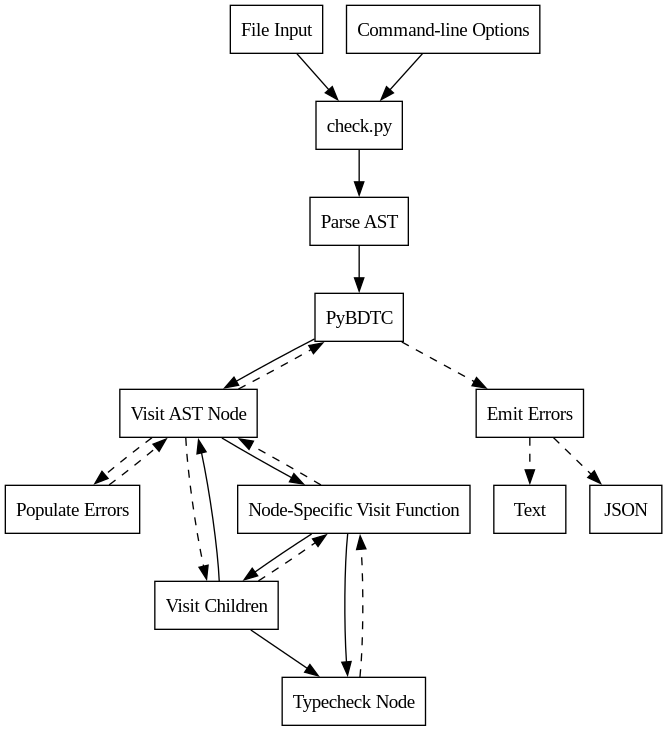
\includegraphics[width=.95\linewidth]{arch.png}
    \caption{
        High-level flow of data. Solid arrows denote context and AST information while dotted arrows denote error information.
    }
    \label{fig:architecture}
\end{figure}

A diagram of the code architecture is shown in Figure \ref{fig:architecture}. The core of the program are the \verb|visit_*| functions. Each AST node is passed to a top-level \verb|visit| function which then dispatches it to a node-specific visit function. For example, annotated assignments (\verb|ast.AnnAssign|) are dispatched to \verb|visit_AnnAssign|. These functions are defined in the \verb|pybdtc.nodes| folder where they are sorted based on the categories used in the Python \verb|ast| documentation. These visit functions may then recursively call the top-level \verb|visit| function on child nodes. 

There are two main data structures that control the flow of information in the project. The \verb|Context| data structure flows "down" from parent node to child node. New variables are added to the context when they come into scope. When a new scope is reached, a copy of the current context is made which is then modified by the child nodes. After the child nodes return, the old context returns, deleting everything that is no longer in scope. 

The \verb|Errors| data structure flows "up" from the child nodes to the parent nodes. Each \verb|visit| function has its own \verb|Errors| data structure that it hen adds its errors to. This data structure is then returned by the \verb|visit| functions where it is then merged into the parent node's visit functions. When it is possible to do so, the errors are populated with filenames and line numbers to provide context as to where the error is occurring. When the program terminates, the final \verb|Errors| data structure contains all of the consolidated type errors encountered in the program and may emit them in the format of the user's choice.
\printbibliography

\end{document}
